\documentclass{article}
\usepackage[UTF8]{ctex}
\usepackage{graphicx}
\usepackage{wrapfig}
\graphicspath{{figure/}}
\begin{document}
村正,可视为一类日本刀的名字,别名为千子村正,在伊势国桑名(现今的三重县桑名市)为一族活跃刀匠的名字,当时村正家族所铸造的刀均称为村正,后因历史原因也出现一些名为村正的日本刀。\par

在德川家还是用三河地区“松平”的姓氏之时,德川家康的祖父松平清康在天文4年(1535)年尾,与织田家作战时被家臣阿部弥七郎用村正刀“千子村正”砍死。相传当时是由右肩斩至左腹。\par

\zihao{5}

\begin{wrapfigure}{r}{4.5cm}
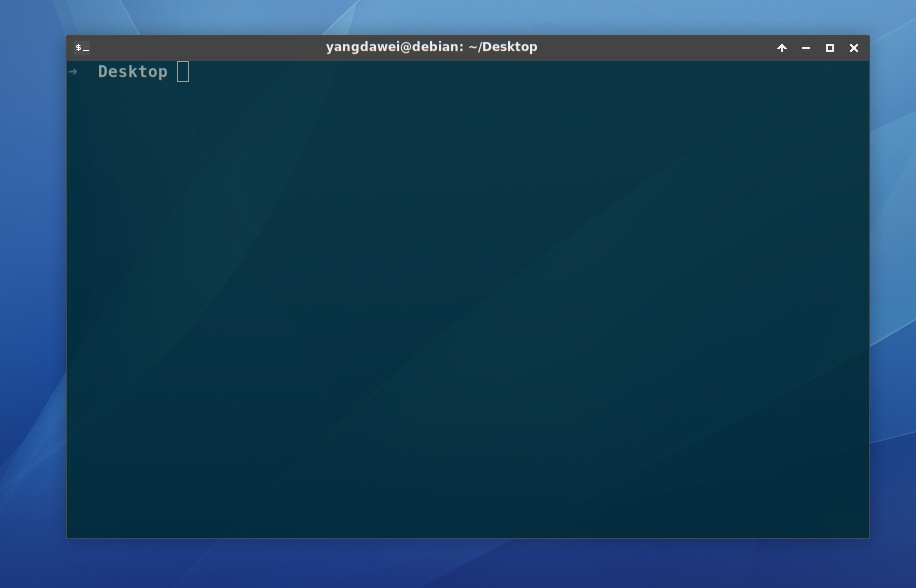
\includegraphics [width=4cm,clip]{cun_c.png}
\caption{my table}
\end{wrapfigure}

在德川家还是用三河地区“松平”的姓氏之时,德川家康的祖父松平清康在天文4年(1535)年尾,与织田家作战时被家臣阿部弥七郎用村正刀“千子村正”砍死。相传当时是由右肩斩至左腹。\par

【“妖刀村正”的传说】\par
\end{document}
%%% Local Variables:
%%% mode: latex
%%% TeX-master: t
%%% End:
